% \documentclass[a4paper]{article}
\documentclass[12pt]{extarticle}
\usepackage[a4paper, left=1.5cm, right=1.5cm, top=1.5cm, bottom=2.0cm]{geometry}
\usepackage{graphicx} % Required for inserting images
\usepackage{caption}  % for continuedfloat

\usepackage{lscape} % For landscape pages
\usepackage{afterpage}
\usepackage{pdflscape} % To create landscape pages that show as landscape in PDF viewer
\usepackage{parskip} % Adds white space between paragraphs


\title{stroke\_lsoa\_prediction}
\author{Anna Laws}
\date{March 2025}

\begin{document}

\maketitle

\section{Introduction}

Columns in the data:

\begin{itemize}
    \item MSOA name and code
    \item Admissions
    \item IMD 2019 Score
    \item Total population of MSOA
    \item Numbers of patients in each health band (good, fair, bad)
    \item Proportions of patients in each health band (good, fair, bad)
    \item Age band proportions (less than 65, 65--70, 70--75, 75--80, over 80)
\end{itemize}

Remove the Welsh MSOA because admissions are always zero.


\section{Check data}
\subsection{Age vs health}

\begin{figure}
    \centering
    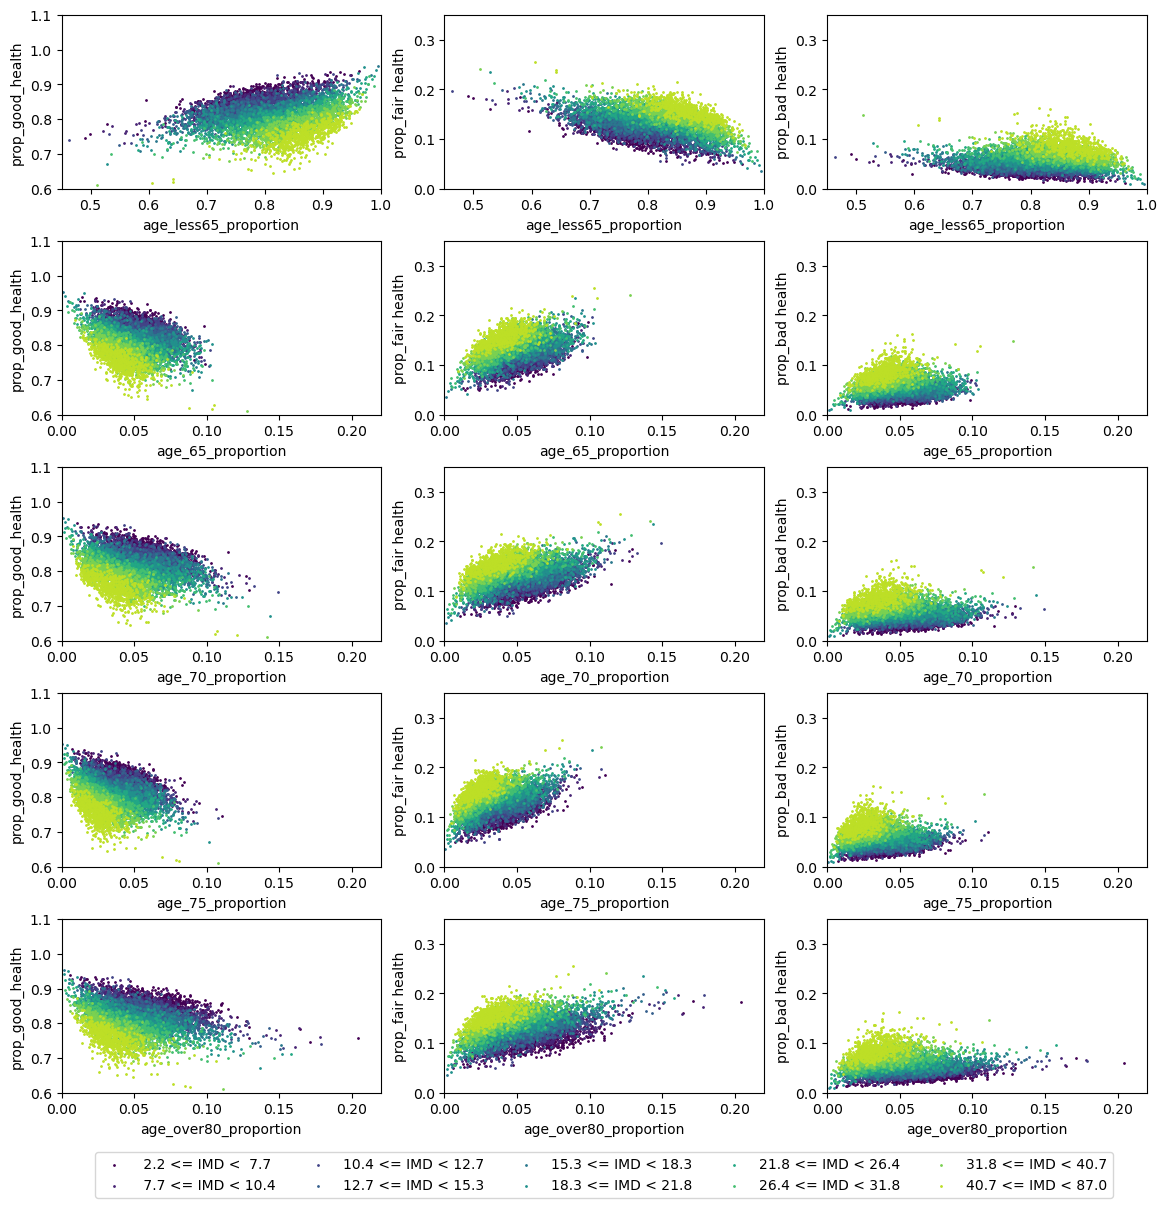
\includegraphics[width=1\linewidth]{images/scatter_age_health_all_by_imd.png}
    \caption{Scatter plots of all age proportions against all health proportions coloured by IMD quantile.}
    \label{fig:data_all_age_health_by_imd}
\end{figure}


\begin{figure}
    \centering
    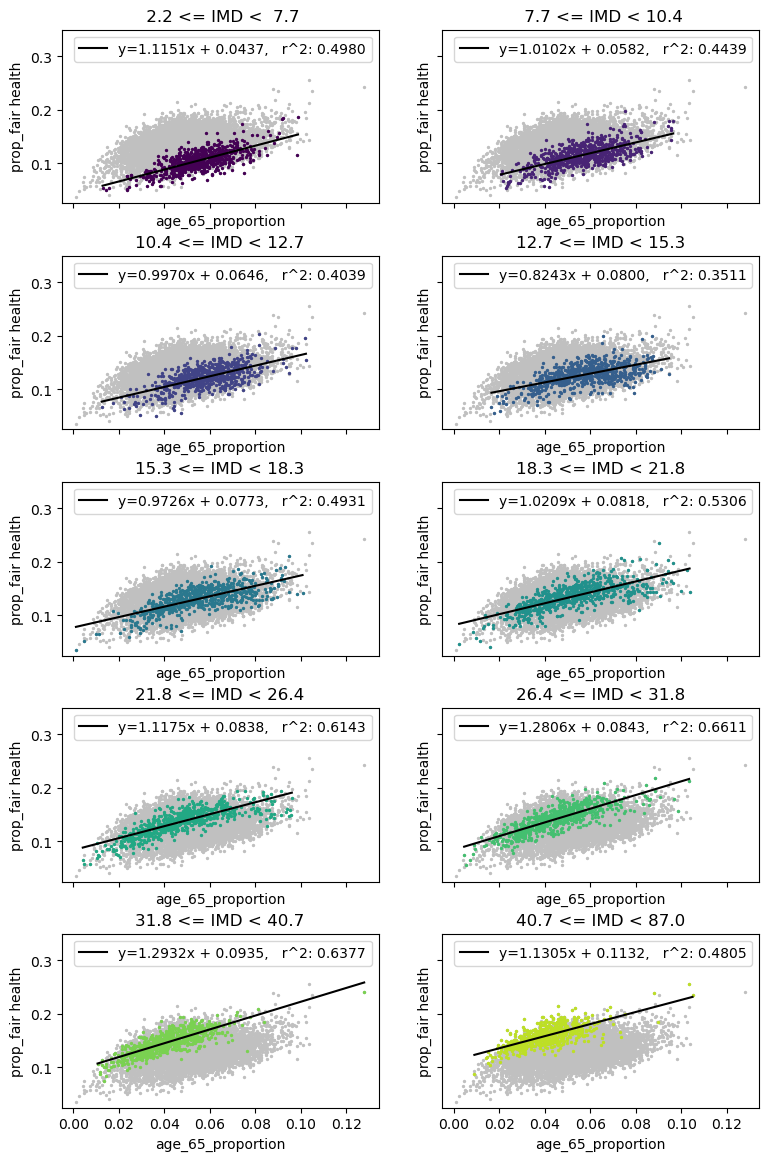
\includegraphics[width=0.8\linewidth]{images/scatter_age_65_proportion_prop_fair health_by_imd.png}
    \caption{Scatter plots of proportion of population aged 65-70 against proportion of population with ``fair'' health for each IMD quantile separately. Data for the specified IMD quantile is shown in colour and all other data is shown in grey.}
    \label{fig:data_example_age_health_by_imd}
\end{figure}

Figure~\ref{fig:data_all_age_health_by_imd} shows scatter plots of each age band against each health proportion.
Generally as the proportions of patients in the higher age band increases, the proportion of patients in good health decreases and the proportion of patients in fair or bad health increases.
The relation is not too clear when considering all English MSOA at once: most points would lie some distance away from a linear regression line of best fit.

When the data is split into ten IMD quantiles, MSOA with similar IMD scores show a tighter correlation between the health and age proportions.
In Figure~\ref{fig:data_example_age_health_by_imd} the proportion of the population with fair health is shown against the proportion of patients in the 65-70 age band, and patients in each IMD band are highlighted separately in each plot.
The data for each IMD band follows a linear regression fit with less variance around the line than when all IMD bands were considered together.
The IMD bands occupy different parts of the whole dataset (shown in grey).
For a fixed age proportion, e.g. proportion with age 65--70 = 0.06, the lower IMD (less deprived) areas tend to have a lower proportion of patients in fair health than the higher IMD areas.

Use IMD score splits that make 10\% quantiles. The first IMD split contains the 10\% least deprived MSOAs, the next split contains the 10\%-20\% least deprived, etc. until the last group contains the top 10\% most deprived MSOAs.


\subsection{Health vs admissions}

\begin{figure}[!b]
    \centering
    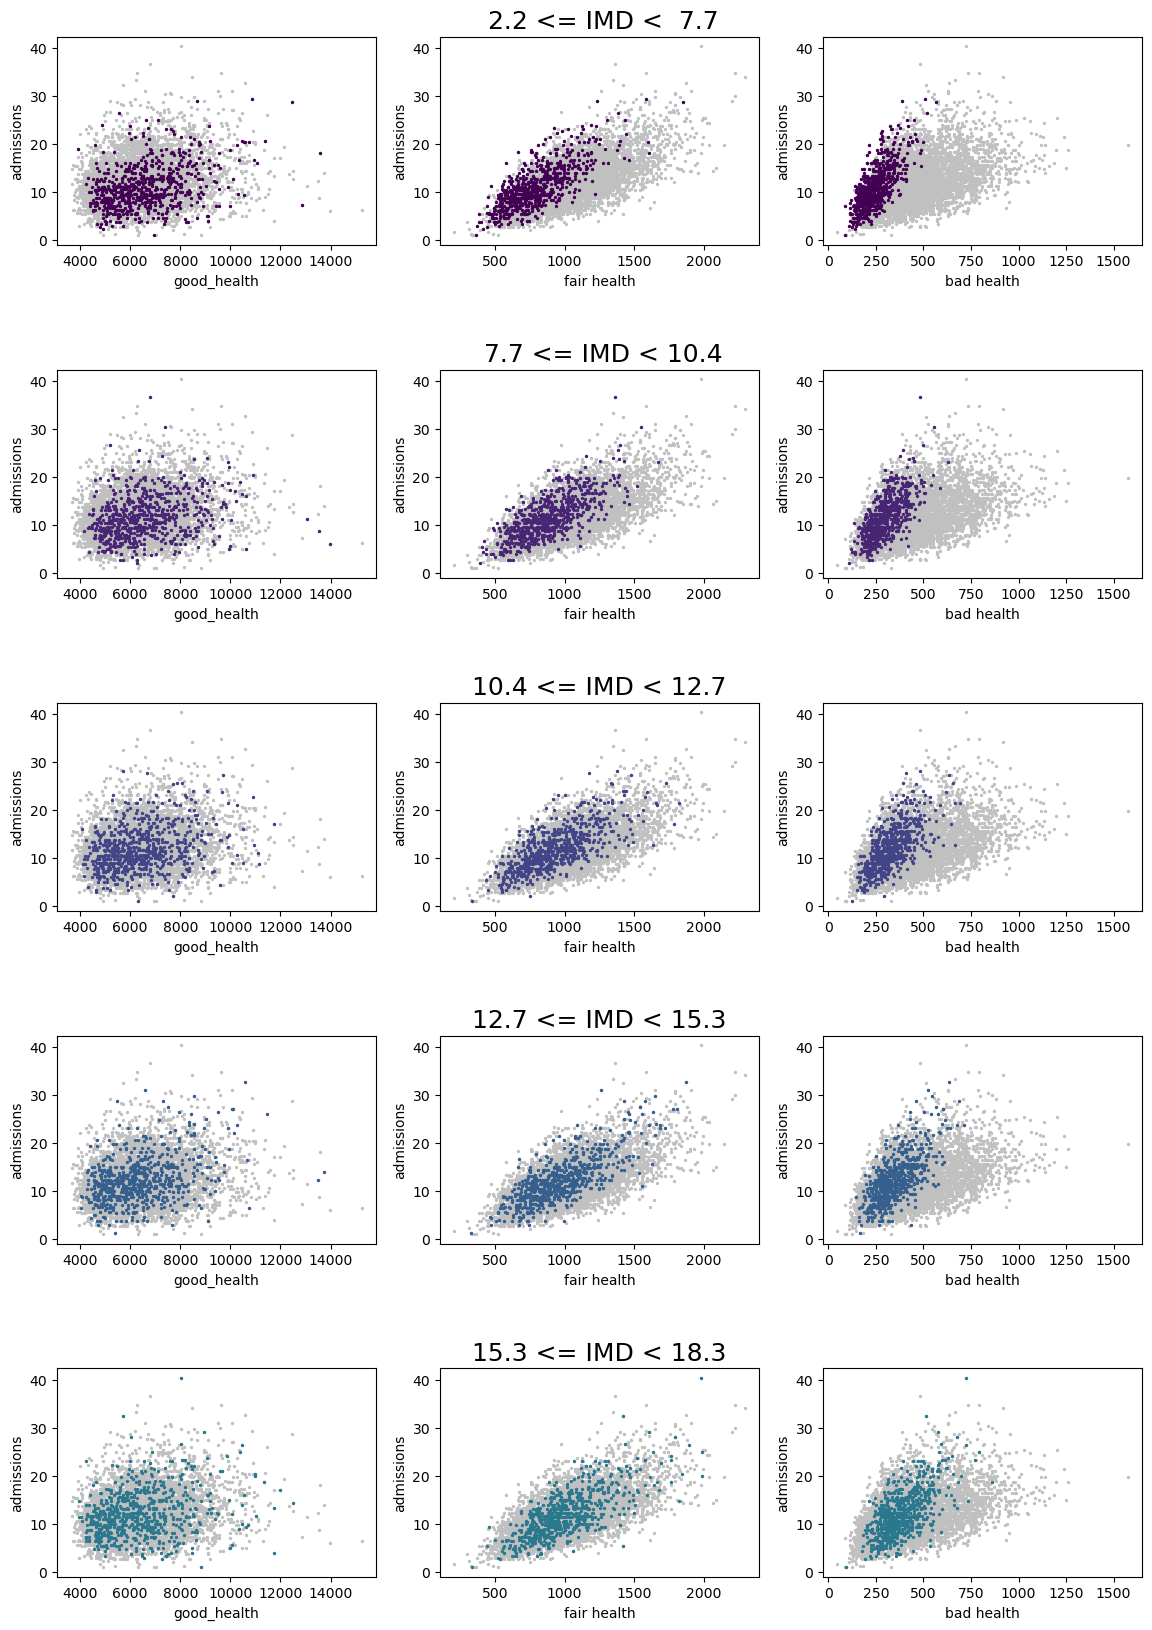
\includegraphics[width=0.9\linewidth]{images/scatter_health_admissions_by_imd_0.png}
    \caption{(Part 1 of 2) Scatter plots of *numbers* of good/fair/bad health against admissions for each IMD quantile separately. Data for the specified IMD quantile is shown in colour and all other data is shown in grey.}
    % don't label this figure to keep same figure number as following.
\end{figure}

\begin{figure}[ht]\ContinuedFloat  % don't make a new figure number
    \centering
    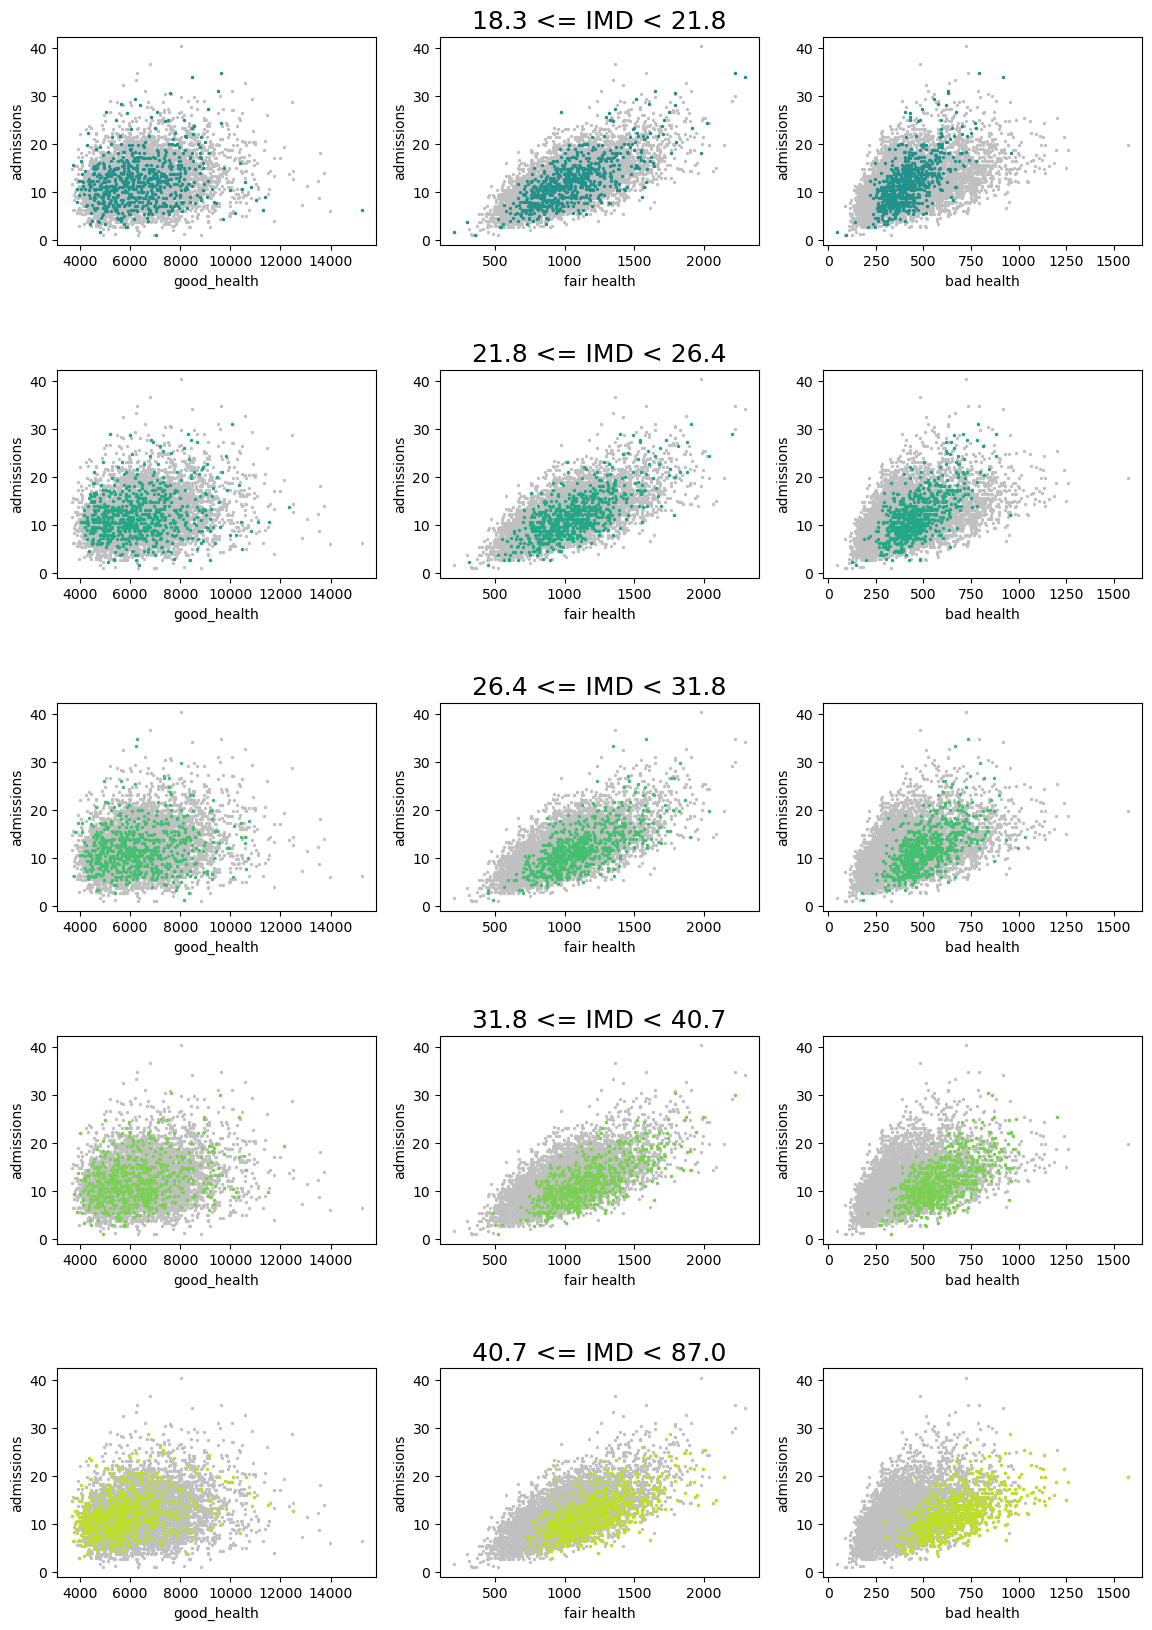
\includegraphics[width=0.9\linewidth]{images/scatter_health_admissions_by_imd_1.png}
    \caption{(Part 2 of 2) Scatter plots of *numbers* of good/fair/bad health against admissions for each IMD quantile separately. Data for the specified IMD quantile is shown in colour and all other data is shown in grey.}
    \label{fig:data_health_admissions_by_imd}
\end{figure}
\clearpage

When comparing *numbers* (not proportions) of patients with each health state with the number of admissions, there should be a trend of larger MSOAs having more stroke admissions based only on having a higher population.
In Figure~\ref{fig:data_health_admissions_by_imd} there is not much correlation between the *number* of patients with good health and the number of admissions for any of the IMD bands.
However the *numbers* of patients with fair health and bad health increase with the numbers of stroke admissions, and the trends differ by IMD band in a similar way to the health vs age proportions graphs.
Here, for the same *number* of patients in fair health (e.g. 1000 patients), the number of admissions is higher for areas with the lowest IMD (least deprived).
The same effect is seen when instead plotting the *proportion* of patients in fair health against the *proportion* of admissions from the MSOA population.

?? Maybe in higher IMD, younger people are more likely to have poor/bad health and also less likely to have strokes due to their age?


\section{Fit lines to data}

\subsection{Predict health from age}


\begin{figure}
    \centering
    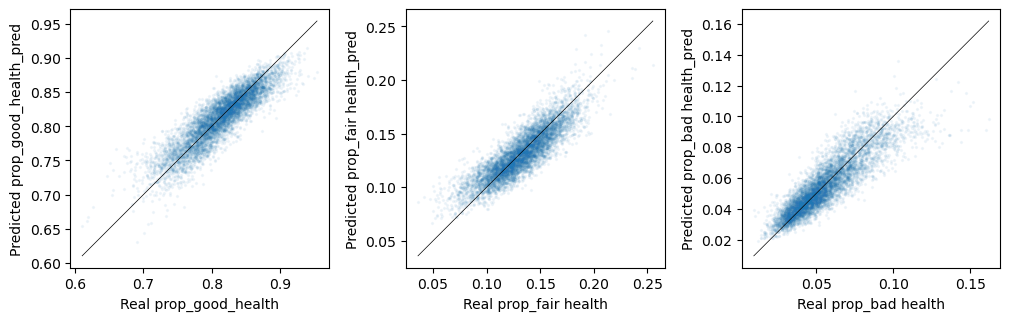
\includegraphics[width=1.0\linewidth]{images/health_scatter_predicted_vs_real_from_real_age_props.png}
    \caption{Real vs predicted health proportions using the real proportions of patients in each age band. The lines are $y=x$.}
    \label{fig:health_predicted_from_real_age_props}
\end{figure}

Each age band proportion is fitted to each health proportion independently, i.e. good, poor and bad health are considered separately.
The model fit is a linear regression with a constant to find the coefficients in $p_h = m_a \cdot p_a + c_a$ for a health proportion $p_h$, age proportion $p_a$, age coefficient $m_a$, and constant $c_a$.
We find a different combination of $m_a$ and $c_a$ for each combination of age band proportion (under 65, 65--70, 70--75, 75--80, over 80), health proportion (good, poor, bad health), and IMD quantile.
The line fit is found using the ordinary least squares (OLS) model from the `statsmodels` package.

Figure~\ref{fig:health_predicted_from_real_age_props} shows the health proportions predicted using the fitted health-vs-age lines with the real proportions of people in each age band.

\subsection{Predict admissions from health}

\begin{figure}
    \centering
    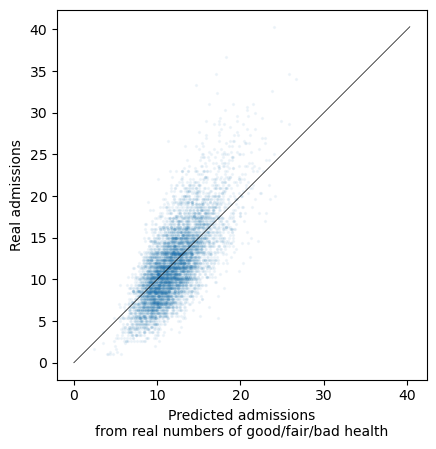
\includegraphics[width=0.5\linewidth]{images/admissions_scatter_predicted_vs_real_from_real_health_props.png}
    \caption{Real vs predicted admissions using the real numbers of patients in good, poor, and bad health conditions. The line is $y=x$.}
    \label{fig:admissions_predicted_from_real_health_props}
\end{figure}

The three health groups are used together to predict the number of admissions.
The number of people in each health band is scaled by a coefficient and the three values are summed.
The resulting admissions $a = c_g \cdot n_g + c_p \cdot n_p + c_b \cdot n_b$ for admissions $a$ and coefficients $c$ and numbers of people $n$ for good $g$, poor $p$, and bad $b$ health.
There is no constant in this equation so that when the numbers of people with good, poor or bad health are zero, the number of admissions is zero.
The coefficients $c$ are forced to lie between 0 and 1 so that they act as the probability of having a stroke for a person in that health group, e.g. $c_g = P(\textnormal{stroke} | \textnormal{good health})$.

The best values for the coefficients $c_g$, $c_p$ and $c_b$ are fitted for each IMD group separately using the `scipy` package's `optimize.minimize` function.


\begin{table}
\centering
\caption{Coefficients for predicting admissions from health proportions.}
\begin{tabular}{l l l l l l}
imd\_bin\_min & imd\_bin\_max & coeff\_good\_health & coeff\_fair\_health & coeff\_bad\_health & rsquared \\
f64 & f64 & f64 & f64 & f64 & f64 \\

2.2122 & 7.708 & 0.0 & 0.008549 & 0.017694 & 0.5722268 \\
7.708 & 10.369 & 0.0 & 0.0101521 & 0.0091246 & 0.5156227 \\
10.369 & 12.74375 & 0.0 & 0.0118571 & 0.0027425 & 0.5254204 \\
12.74375 & 15.2564 & 0.0 & 0.0119053 & 0.0023227 & 0.565176 \\
15.2564 & 18.32929 & 0.0 & 0.0121379 & 0.0 & 0.5270501 \\
18.32929 & 21.81475 & 0.0 & 0.0116203 & 0.0000015 & 0.5140601 \\
21.81475 & 26.36117 & 0.0 & 0.0110406 & 0.0006057 & 0.4988284 \\
26.36117 & 31.84075 & 0.0 & 0.0093152 & 0.0031409 & 0.461555 \\
31.84075 & 40.6996 & 0.0 & 0.0082107 & 0.0040624 & 0.4981876 \\
40.6996 & 87.02675 & 0.0 & 0.0067975 & 0.0056979 & 0.4132969 \\

\end{tabular}
\label{tab:coeffs_admissions_from_health}
\end{table}


Figure~\ref{fig:admissions_predicted_from_real_health_props} shows the admission numbers predicted using the fitted admissions-vs-health lines with the real numbers of people in each health category.

\subsection{Steps for predicting admissions from age}

\begin{itemize}
    \item Group MSOAs by their IMD score. 
    \item Take proportions of population in each age band (under 65, 65--70, 70--75, 75--80, over 80).
    \item Use the health-age-IMD line fits to calculate new proportions of patients with good, poor and bad health from the age band proportions.
    \item Use the total population of the MSOA to scale the health proportions to health numbers.
    \item Use the admissions-health-IMD line fits to calculate new admission numbers from the new health numbers.    
\end{itemize}

\section{Results}

\subsection{Predict admissions from age proportions}

\begin{figure}
    \centering
    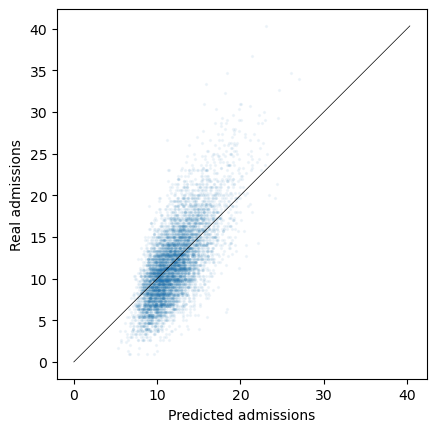
\includegraphics[width=0.5\linewidth]{images/admissions_scatter_predicted_vs_real_from_real_age_props.png}
    \caption{Real vs predicted admissions using the real proportions of patients in each age band. The line is $y=x$.}
    \label{fig:admissions_predicted_from_real_age_props}
\end{figure}

Figure~\ref{fig:admissions_predicted_from_real_age_props} shows the admission numbers predicted using the fitted health-vs-age then admissions-vs-health lines with the real proportions of people in each age band.


\section{Alternative method}


\begin{figure}[!b]
    \centering
    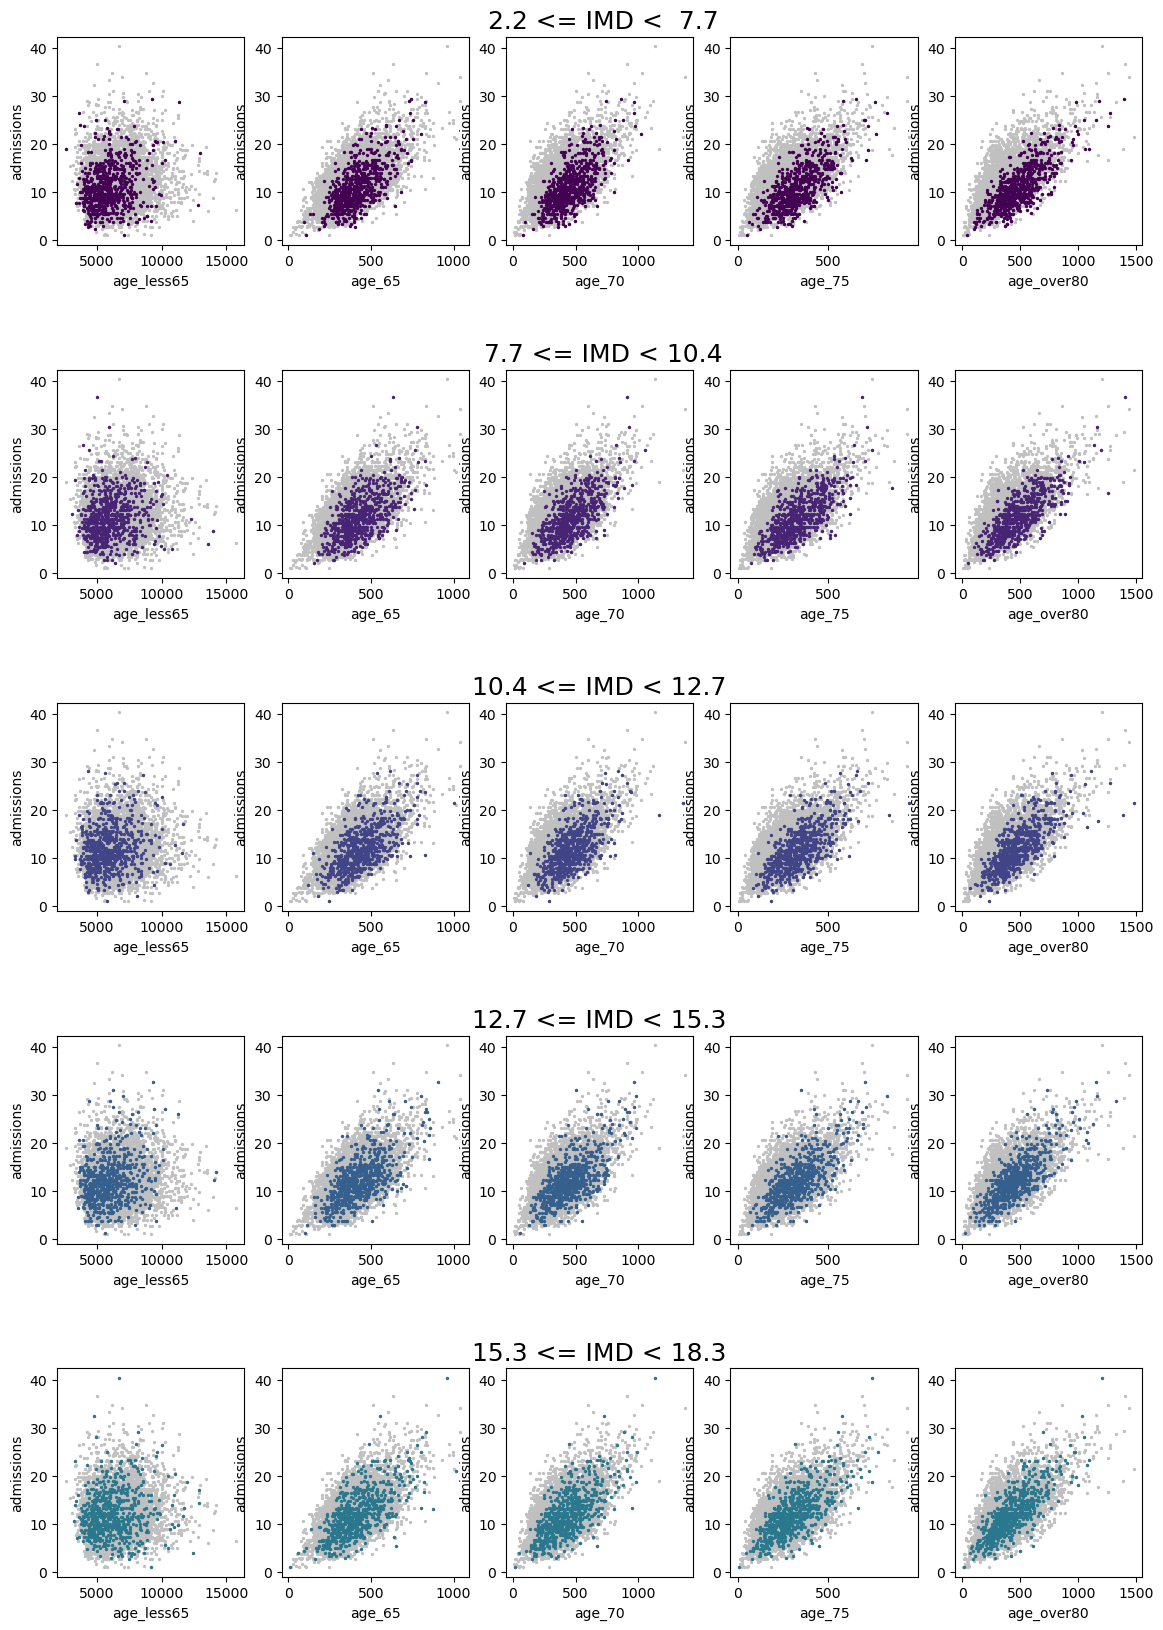
\includegraphics[width=0.9\linewidth]{images/scatter_age_admissions_by_imd_0.png}
    \caption{(Part 1 of 2) Scatter plots of proportions in each age band against admissions for each IMD quantile separately. Data for the specified IMD quantile is shown in colour and all other data is shown in grey.}
    % don't label this figure to keep same figure number as following.
\end{figure}

\begin{figure}[ht]\ContinuedFloat  % don't make a new figure number
    \centering
    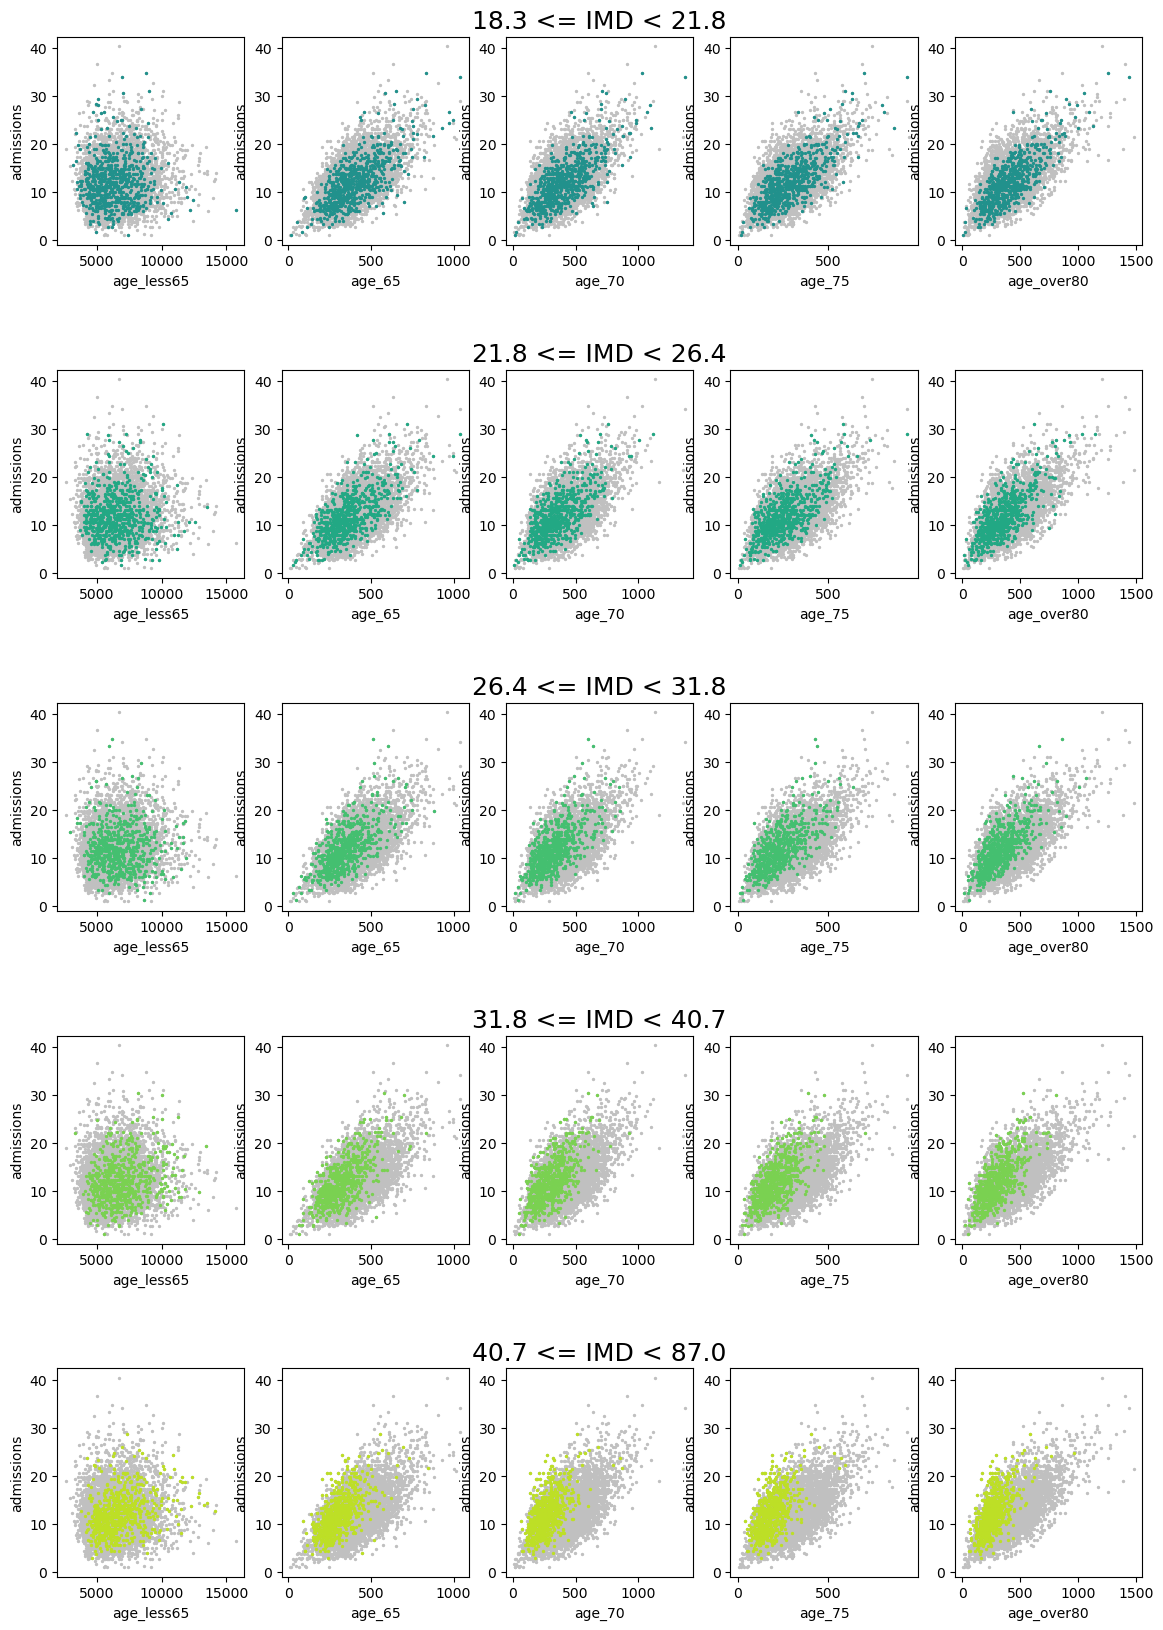
\includegraphics[width=0.9\linewidth]{images/scatter_age_admissions_by_imd_1.png}
    \caption{(Part 2 of 2) Scatter plots of proportions in each age band against admissions for each IMD quantile separately. Data for the specified IMD quantile is shown in colour and all other data is shown in grey.}
    \label{fig:data_age_admissions_by_imd}
\end{figure}
\clearpage

\subsection{Predict admissions from age, skipping health}

\begin{figure}
    \centering
    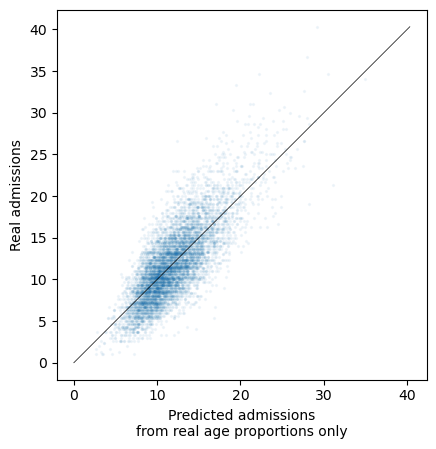
\includegraphics[width=0.5\linewidth]{images/admissions_scatter_predicted_vs_real_from_real_age_props_only.png}
    \caption{Real vs predicted admissions using *only* the real proportions of patients in each age band, skipping the health proportions. The line is $y=x$.}
    \label{fig:admissions_predicted_from_real_age_props_only}
\end{figure}

Skip the health predictions and just use age split by IMD to predict admissions.



The data shows a similar trend with IMD band for age proportions vs admissions (Figure~\ref{fig:data_age_admissions_by_imd}) as there is for health proportions vs admissions (Figure~\ref{fig:data_health_admissions_by_imd}).
For a fixed proportion of a given age band, the number of admissions tends to be higher for higher IMD bands (more deprivation).


The age bands are used together to predict the number of admissions.
The *number* of people in each age band is scaled by a coefficient and the three values are summed.
The resulting admissions $a = \Sigma c_a \cdot n_a$ for admissions $a$ and coefficients $c$ and numbers of people $n$ in each age band $a$.
There is no constant in this equation so that when the numbers of people in all age bands are zero, the number of admissions is zero.
The coefficients $c$ are forced to lie between 0 and 1 so that they act as the probability of having a stroke for a person in that age band, e.g. $c_{a=65} = P(\textnormal{stroke} | \textnormal{age=65--70})$.

The best values for the coefficients $c_a$ are fitted for each IMD group separately using the `scipy` package's `optimize.minimize` function.


\afterpage{%
    \clearpage% Flush earlier floats (otherwise order might not be correct)
    \thispagestyle{empty}% empty page style (?)
    \begin{landscape}% Landscape page
        \centering % Center table
\begin{table}
\centering
\caption{Coefficients for predicting admissions from age proportions only.}
\begin{tabular}{l l l l l l l l}
imd\_bin\_min & imd\_bin\_max & coeff\_age\_less65 & coeff\_age\_65 & coeff\_age\_70 & coeff\_age\_75 & coeff\_age\_over80 & rsquared \\
f64 & f64 & f64 & f64 & f64 & f64 & f64 & f64 \\

2.2122 & 7.708 & 0.000216 & 0.0045511 & 0.0004222 & 0.0001681 & 0.015805 & 0.6405077 \\
7.708 & 10.369 & 0.0002804 & 0.0006162 & 0.0036581 & 0.0017267 & 0.0153756 & 0.6219353 \\
10.369 & 12.74375 & 0.0004032 & 0.0 & 0.0010067 & 0.0060946 & 0.0147307 & 0.5826284 \\
12.74375 & 15.2564 & 0.0004168 & 0.002319 & 0.0009812 & 0.0037331 & 0.0156056 & 0.6544553 \\
15.2564 & 18.32929 & 0.000354 & 0.003684 & 0.0000001 & 0.0016998 & 0.0182403 & 0.6407842 \\
18.32929 & 21.81475 & 0.0004139 & 0.0020376 & 0.0014869 & 0.0060625 & 0.0154113 & 0.6564009 \\
21.81475 & 26.36117 & 0.0005089 & 0.0043913 & 0.0051061 & 0.0 & 0.0144993 & 0.5971861 \\
26.36117 & 31.84075 & 0.0004742 & 0.0063397 & 0.0003535 & 0.0035603 & 0.016621 & 0.5776872 \\
31.84075 & 40.6996 & 0.0005902 & 0.0 & 0.0071645 & 0.0016448 & 0.0179369 & 0.5592986 \\
40.6996 & 87.02675 & 0.0006674 & 0.004432 & 0.0092856 & 0.0000004 & 0.0143878 & 0.4766468 \\

\end{tabular}
\label{tab:coeffs_admissions_from_age_only}
\end{table}
    \end{landscape}
    \clearpage% Flush page
}

Steps:
\begin{itemize}
    \item Group MSOAs by their IMD score. 
    \item Take proportions of population in each age band (under 65, 65--70, 70--75, 75--80, over 80).
    \item Use the admissions-age-IMD line fits to calculate new admission numbers from the new health numbers.    
\end{itemize}


Figure~\ref{fig:admissions_predicted_from_real_age_props_only} shows the admission numbers predicted using the fitted admissions-vs-age lines with the real proportions of people in each age band.


\end{document}
